\section{\todo{Particle Accelerators and CERN}}

\subsection{\todo{Particle Accelerators}}

%The first modern particle accelerators started to be conceived at the beginning of the 1900s. Those
%first accelerators, such as the Cockroft-Walton generator, used voltage multipliers to generate
%electric fields in order to accelerate particles.  Voltage multipliers are nowadays still an
%important piece of equipment as they are used in devices requiring high voltage, such as X-Ray
%machines, CRT monitors, microwaves or as part of an accelerator complex.  Those early technologies
%were namely used to perform the first artificial nuclear disintegration.

\lipsum[1]

\subsection{\todo{The CERN Complex}}

\lipsum[1]


% ===============================
%             LHC
% ===============================
\subsection{\review{The Large Hadron Collider}}

The Large Hadron Collider (LHC), is a circular particle accelerator primarily designed to collide
protons for fundamental particle physics research. It can, occasionally over the year, also collide
ions such as oxygen or lead for specifics studies. At the time of writing, in 2024, it holds several
records, such as being the largest and most powerful accelerator in the world. The LHC is composed
of two beams pipes, being able to accelerate two particle beams from an injection energy of $450$GeV
to an energy of $6,800$GeV, before colliding them in four detectors: ATLAS, CMS, Alice and LCHb.

Well publicized, the LHC is often depicted via its superconducting dipole magnets, housed in a blue
cryostat, aimed at cooling the coils. \cref{fig:3d_cut_dipole} shows a 3D cut of such magnets. The
LHC is in majority composed of those \textit{main} dipoles, as it holds $1,232$ of them, being each
about 14 meters long. Superconducting materials like Niobium-Titanium (NbTi) are utilized, as
conventional materials such as copper would melt under the current strain. There are indeed around
$12,000$ amperes supplied to generate the magnetic fields necessary for bending the trajectory of
the particles.
Those particles travel at nearly the speed of light (more precisely, $99.99999905\%$ of it),
effectively going around the tunnel about $11,200$ times per second.

\begin{figure}[!htb]
    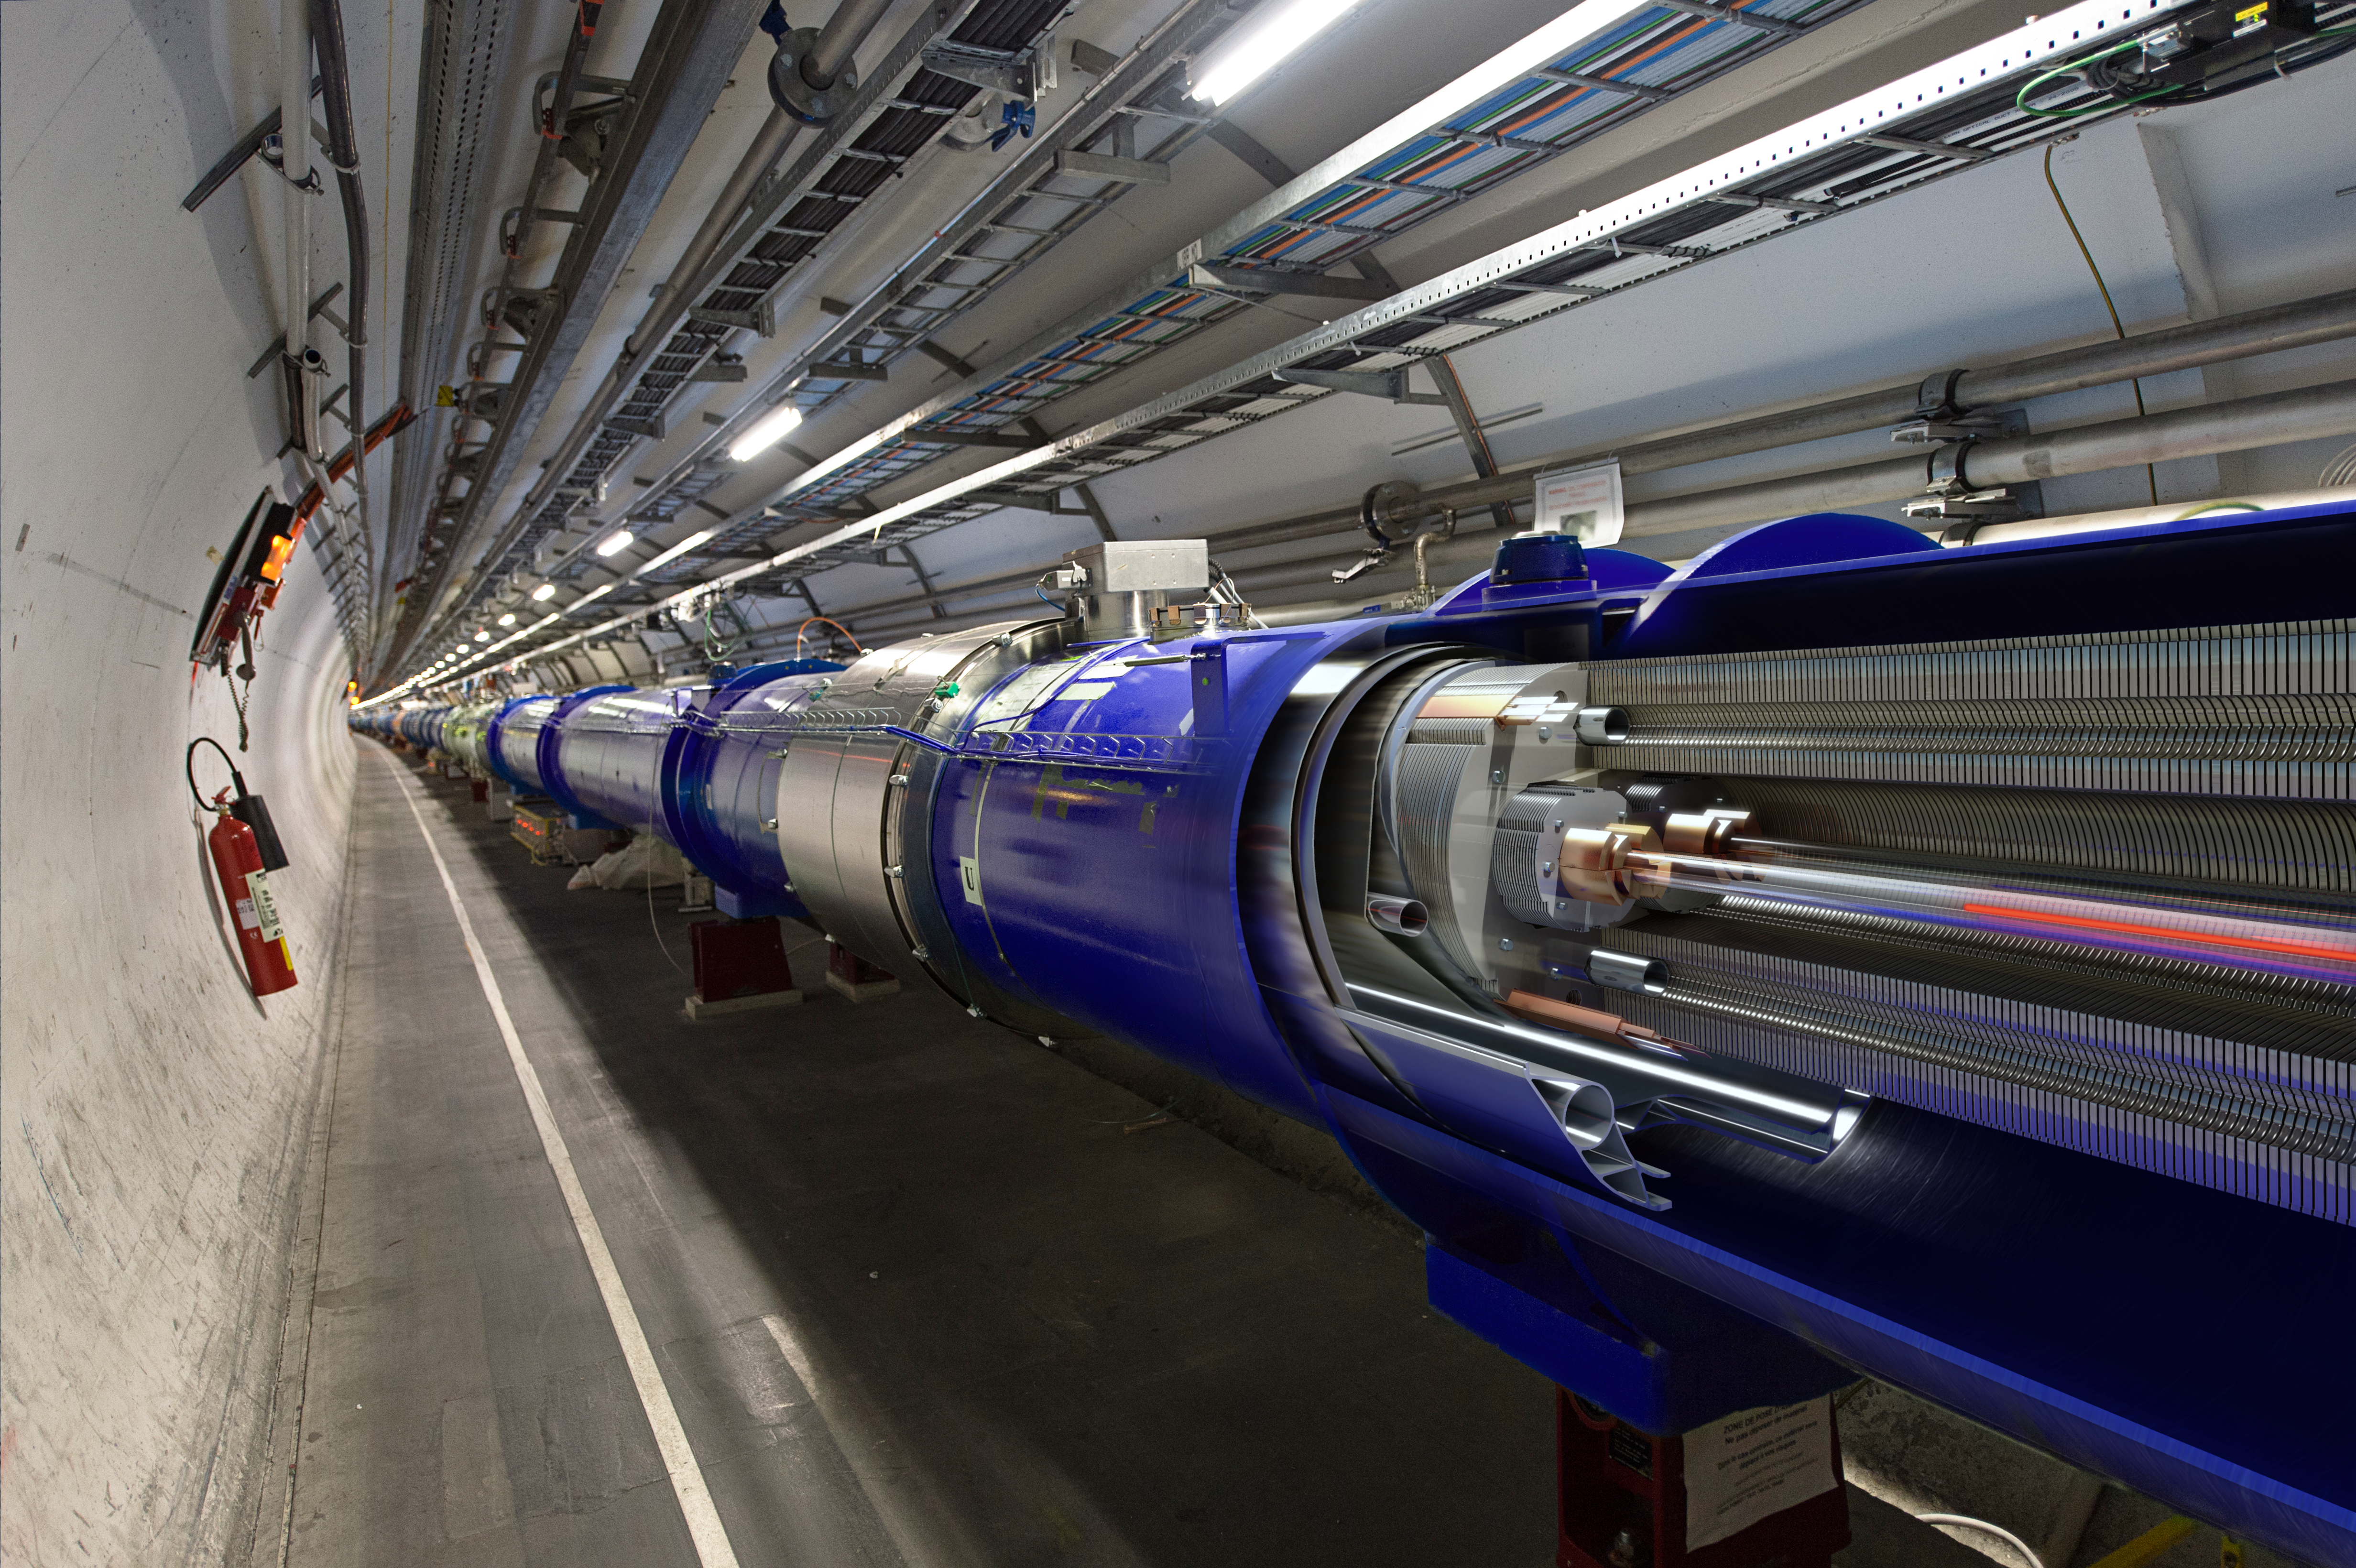
\includegraphics[width=\textwidth]{chapters/01_Introduction/images/lhc_3D_cut.png}
    \caption{3D cut of a main LHC dipole~\cite{noauthor_cern_nodate}. Both beam pipes can be seen
    surrounded by the coils, strongly clamped by the yokes.}
    \label{fig:3d_cut_dipole}
\end{figure}


\paragraph{Straight Sections and Arcs}
The LHC is not a perfect circle. It is indeed composed of four \textit{straight} sections, called
the \textit{Interaction Regions} (IPs) where detectors or instrumentation are placed. Connecting
those sections, the \textit{arcs} are where the majority of the magnets are placed, housing dipoles,
quadrupoles, sextupoles, octupoles and their respective correctors. \cref{fig:introduction:lhc_irs}
shows how the instrumentation, detectors and arcs are distributed along the ring.

\begin{figure}[!htb]
    \centering
    \includegraphics[width=0.5\textwidth]{./images/irs.png}
    \caption{Schematic of the LHC layout.}
    \label{fig:introduction:lhc_irs}
\end{figure}


\paragraph{Arc Cells}

Each arc is made up of 23 cells. Magnets are organized in a standard FoDo structure
(see \ref{section:courant_snyder}), as shows \cref{fig:introduction:lhc_arc_cell}.
\textit{Dipoles} are responsible for bending the trajectory of the particles. Their associated
correctors, the orbit correctors, mitigate any possible drift in path.
\textit{Quadrupoles} are used to control the beam size along the ring. Their effect is focusing in
one plane and defocusing in the other. Their associated correctors control the oscillations of the
beam (see tune, \ref{section:courant_snyder}) and possible field imperfections.
\textit{Sextupoles} correct chromaticity, being a misfocus from quadrupoles due to particles having
a different momentum than the reference particle.
\textit{Octupoles} are used to stabilize the beam by introducing Landau
Damping~\cite{gareyte_landau_1997}. The associated correctors correct higher order chromaticity
effects as well as amplitude dependant tune shifts.
\textit{Decapoles} correctors aim at correcting even a higher chromaticity order.

\begin{figure}[H]
    \centering
    \includegraphics[width=1\textwidth]{./images/lhc_cell.png}
    \caption{Schematic of an LHC Arc cell~\cite{bruning_lhc_2004}.}
    \label{fig:introduction:lhc_arc_cell}
\end{figure}



% ===============================
%          Parameters
\subsubsection{\review{Parameters}}

During the operation of the LHC, the machine goes through several states. Those states of the
machine~\cite{wenniger_lhc_2019} have been defined for specific scenarios.

A common example is the operational cycle of the LHC, shown in \cref{fig:cern_complex:cycle}.
The magnets are first pre-cycled~\cite{bottura_pre-cycles_2010} without any beam circulating, to get
them back to a reproducible state. Their current is then increased to accept particles at the 
injection energy of 450GeV. In order to assess the good working condition of the machine, a probe
bunch of reduced intensity is injected first. The number of bunches and their intensity is then
ramped up to attain the desired scheme needed for collisions. This scheme varies throughout the year
depending on the demands of the experiments. The number of bunches and intensity can also be lowered
for to keep the machine safe. A common scheme in 2024 is to inject about 2350 bunches with around
$10^{11}$ particles each for collisions.
Optics measurements, due to their destructive nature, typically use between one and three
\textit{pilot} bunches at a lower intensity of $10^{10}$.

The magnets current is them ramped along with the voltage injected in the RF system, to 
accelerate particles to an energy of 6.8TeV. While doing so so, the beam is squeezed in a first pass
at the Interaction Points. A second pass is done after the ramp is over, to reach a $\beta* = 30cm$
at the ATLAS and CMS experiments. Crossing-angles are then introduced to make the beams colliding.

\begin{figure}[!htb]
    \includegraphics[width=\textwidth]{./images/lhc_cycle.pdf}
    \caption{Simplified illustration of a standard LHC cycle. Courtesy of Félix
    Soubelet~\cite{felix_soubelet_local_2023}} \label{fig:cern_complex:cycle}
\end{figure}


% ===============================
%   Harmonics and Field Errors
\subsubsection{\review{Harmonics and Field Errors}}

Real-life magnets never have a single field as one would like. Instead, so called 
\textit{allowed harmonics} exist due to the geometry of the coil. As such, the main dipoles of the
LHC can exhibit fields similar to sextupoles, decapoles, decatetrapoles and so
on~\cite{deniau_magnetic_2009}. Manufacturing imperfections also add fields errors outside of the
scope of the allowed ones. Dipoles are indeed found to generate octupolar field errors.

During the design of the LHC, the main dipoles have been identified to generate significant field
errors. Magnetic measurements of those various fields were thus taken and magnetic tables built
based on real-life magnets nowadays installed in the machine. Those magnetic tables, computed for
each LHC configuration by \textit{WISE}~\cite{p_hagen_wise_2006} are used by simulation softwares.
Predictions of field errors and compensating strength for the correctors is computed by the Field
Description for the LHC (\textit{FiDeL}, \cite{noauthor_fidel_2021}). FiDeL is used in the LHC
control system in operation to steer the LHC.

%\begin{figure}[H]
    %\centering
    %\includegraphics[width=0.5\textwidth]{./images/main_dipole_fields.png}
    %\caption{Magnetic field in a dipole magnet~\cite{deniau_magnetic_2009}.}
    %\label{fig:decapoles:magnetic_field_dipole}
%\end{figure}